\documentclass[landscape]{article}
\usepackage[paperwidth=406.4mm,paperheight=228.6mm,margin=7mm]{geometry}
\usepackage[T1]{fontenc}
\usepackage{lmodern}
\usepackage{microtype}
\usepackage{amsmath,amssymb}
\usepackage{tikz}
\usetikzlibrary{arrows.meta,positioning,calc,fit,shapes.geometric,decorations.pathreplacing,patterns,shadows}
\usepackage[most]{tcolorbox}
\usepackage{tabularx,booktabs,array}
\usepackage{enumitem}
\usepackage{xcolor}
\usepackage{ragged2e}
\pagestyle{empty}
\setlength{\parindent}{0pt}
\renewcommand{\familydefault}{\sfdefault}

% ---------- Palette ----------
\definecolor{bg}{HTML}{F7F9FC}
\definecolor{ink}{HTML}{172033}
\definecolor{muted}{HTML}{5E687D}
\definecolor{line}{HTML}{D8DEE9}
\definecolor{dense}{HTML}{4F46E5}
\definecolor{cnn}{HTML}{059669}
\definecolor{rnn}{HTML}{EA580C}
\definecolor{trf}{HTML}{7C3AED}
\definecolor{densebg}{HTML}{EEF2FF}
\definecolor{cnnbg}{HTML}{ECFDF5}
\definecolor{rnnbg}{HTML}{FFF7ED}
\definecolor{trfbg}{HTML}{F5F3FF}
\definecolor{soft}{HTML}{FFFFFF}

\pagecolor{bg}
\color{ink}

% ---------- Reusable styles ----------
\tcbset{
  archbox/.style={
    enhanced,
    arc=4mm,
    boxrule=0.8pt,
    left=2.5mm,right=2.5mm,top=2.2mm,bottom=2.2mm,
    drop shadow={opacity=0.16,shadow xshift=1.5mm,shadow yshift=-1.5mm},
    height=121mm,
    valign=top,
    fontupper=\scriptsize
  },
  sectionbox/.style={
    enhanced,
    arc=2mm,
    boxrule=0pt,
    left=2mm,right=2mm,top=1.4mm,bottom=1.4mm,
    colback=white,
    before skip=1.4mm,after skip=1.4mm,
  }
}

\newcommand{\apptag}[2]{\tikz[baseline=(X.base)]\node[inner xsep=1.7mm,inner ysep=0.55mm,rounded corners=1.2mm,fill=#1!12,text=#1,font=\tiny\bfseries](X){#2};}
\newcommand{\cardtitle}[3]{%
  {\Large\bfseries\color{#1} #2}\hfill\tikz[baseline=-0.6ex]\node[circle,fill=#1,text=white,inner sep=1.45mm,font=\bfseries\scriptsize]{#3};\par
  \vspace{1mm}{\color{muted}\footnotesize #2 architecture}\par\vspace{1mm}\hrule height 0.4pt\color{line}\vspace{1.3mm}
}
\newcommand{\subhead}[2]{\vspace{0.8mm}{\color{#1}\bfseries\scriptsize #2}\par\vspace{0.4mm}}

% ---------- Diagrams ----------
\newcommand{\densedigram}{%
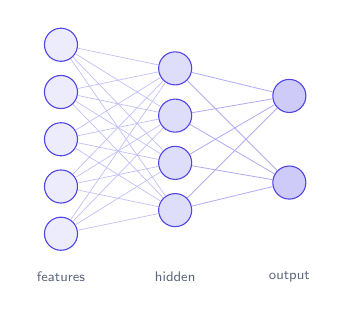
\begin{tikzpicture}[x=1cm,y=1cm,>=Latex, neuron/.style={circle,draw=dense,fill=dense!10,minimum size=4.2mm,inner sep=0pt}, small/.style={font=\tiny,color=muted}]
  \foreach \y/\i in {1.2/1,0.6/2,0/3,-0.6/4,-1.2/5}{\node[neuron] (i\i) at (0,\y) {};}
  \foreach \y/\i in {0.9/1,0.3/2,-0.3/3,-0.9/4}{\node[neuron,draw=dense,fill=dense!18] (h\i) at (1.45,\y) {};}
  \foreach \y/\i in {0.55/1,-0.55/2}{\node[neuron,draw=dense,fill=dense!28] (o\i) at (2.9,\y) {};}
  \foreach \a in {1,...,5}{\foreach \b in {1,...,4}{\draw[dense!35,line width=0.25pt] (i\a)--(h\b);}}
  \foreach \a in {1,...,4}{\foreach \b in {1,2}{\draw[dense!45,line width=0.3pt] (h\a)--(o\b);}}
  \node[small] at (0,-1.75) {features};
  \node[small] at (1.45,-1.75) {hidden};
  \node[small] at (2.9,-1.75) {output};
\end{tikzpicture}}

\newcommand{\cnndigram}{%
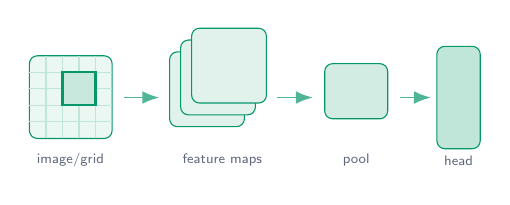
\begin{tikzpicture}[x=1cm,y=1cm,>=Latex, lab/.style={font=\tiny,color=muted}, block/.style={rounded corners=1mm,draw=cnn,fill=cnn!10,line width=0.4pt}]
  \draw[block,fill=cnn!8] (0,0) rectangle (1.05,1.05);
  \foreach \x in {0.21,0.42,0.63,0.84}{\draw[cnn!25] (\x,0)--(\x,1.05); \draw[cnn!25] (0,\x)--(1.05,\x);}
  \draw[draw=cnn,line width=0.8pt,fill=cnn!22] (0.42,0.42) rectangle (0.84,0.84);
  \node[lab] at (0.52,-0.28) {image/grid};
  \draw[-Latex,cnn!70,line width=0.7pt] (1.2,0.52)--(1.65,0.52);
  \foreach \s/\x/\y in {1/1.78/0.15,2/1.92/0.3,3/2.06/0.45}{\draw[block,fill=cnn!12] (\x,\y) rectangle +(0.95,0.95);}
  \node[lab] at (2.45,-0.28) {feature maps};
  \draw[-Latex,cnn!70,line width=0.7pt] (3.15,0.52)--(3.6,0.52);
  \draw[block,fill=cnn!18] (3.75,0.25) rectangle (4.55,0.95);
  \node[lab] at (4.15,-0.28) {pool};
  \draw[-Latex,cnn!70,line width=0.7pt] (4.7,0.52)--(5.1,0.52);
  \node[block,minimum width=0.55cm,minimum height=1.3cm,fill=cnn!25] at (5.45,0.52) {};
  \node[lab] at (5.45,-0.28) {head};
\end{tikzpicture}}

\newcommand{\rnndigram}{%
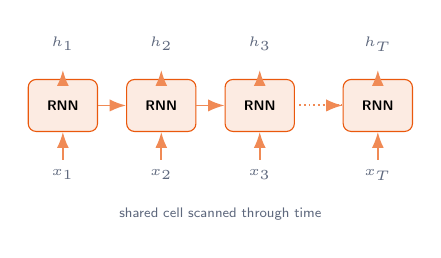
\begin{tikzpicture}[x=1cm,y=1cm,>=Latex, cell/.style={rounded corners=1mm,draw=rnn,fill=rnn!12,minimum width=0.88cm,minimum height=0.66cm,font=\tiny\bfseries}, lab/.style={font=\tiny,color=muted}]
  \foreach \x/\t in {0/1,1.25/2,2.5/3,4.0/T}{
    \node[cell] (c\t) at (\x,0) {RNN};
    \node[lab] (x\t) at (\x,-0.88) {$x_{\t}$};
    \draw[-Latex,rnn!70,line width=0.6pt] (x\t)--(c\t);
    \node[lab] at (\x,0.78) {$h_{\t}$};
    \draw[-Latex,rnn!70,line width=0.6pt] (c\t)--+(0,0.45);
  }
  \draw[-Latex,rnn!70,line width=0.65pt] (c1)--(c2);
  \draw[-Latex,rnn!70,line width=0.65pt] (c2)--(c3);
  \draw[densely dotted,rnn!70,line width=0.7pt] (3.0,0)--(3.55,0);
  \draw[-Latex,rnn!70,line width=0.65pt] (3.55,0)--(cT);
  \node[lab] at (2.0,-1.38) {shared cell scanned through time};
\end{tikzpicture}}

\newcommand{\trfdigram}{%
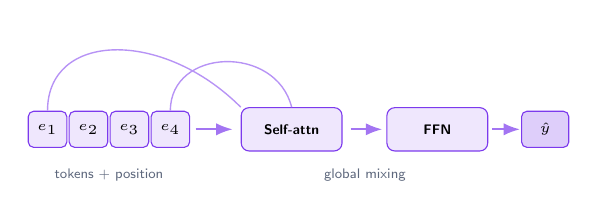
\begin{tikzpicture}[x=1cm,y=1cm,>=Latex, tok/.style={rounded corners=0.7mm,draw=trf,fill=trf!12,minimum width=0.42cm,minimum height=0.46cm,font=\tiny}, block/.style={rounded corners=1mm,draw=trf,fill=trf!12,minimum width=1.28cm,minimum height=0.55cm,font=\tiny\bfseries}, lab/.style={font=\tiny,color=muted}]
  \foreach \x/\n in {0/1,0.52/2,1.04/3,1.56/4}{\node[tok] (t\n) at (\x,0) {$e_\n$};}
  \draw[-Latex,trf!70,line width=0.65pt] (1.88,0)--(2.35,0);
  \node[block] (attn) at (3.1,0) {Self-attn};
  \draw[-Latex,trf!70,line width=0.65pt] (3.85,0)--(4.25,0);
  \node[block] (ffn) at (4.95,0) {FFN};
  \draw[-Latex,trf!70,line width=0.65pt] (5.65,0)--(6.0,0);
  \node[tok,fill=trf!25,minimum width=0.6cm] at (6.32,0) {$\hat y$};
  \draw[trf!55,line width=0.5pt] (t1.north) .. controls +(0,1.0) and +(-1.0,1.0) .. (attn.north west);
  \draw[trf!55,line width=0.5pt] (t4.north) .. controls +(0,0.8) and +(-0.2,0.8) .. (attn.north);
  \node[lab] at (0.78,-0.58) {tokens + position};
  \node[lab] at (4.03,-0.58) {global mixing};
\end{tikzpicture}}

\begin{document}

% ---------- Header ----------
\begin{tcolorbox}[enhanced,arc=4mm,boxrule=0pt,colback=ink,left=6mm,right=6mm,top=4mm,bottom=4mm]
\begin{minipage}[c]{0.67\linewidth}
  {\color{white}\fontsize{24}{28}\selectfont\bfseries Deep Learning Architectures}\par
  \vspace{1mm}
  {\color{white!78}\large Dense $\cdot$ Convolutional $\cdot$ Recurrent $\cdot$ Transformer}
\end{minipage}\hfill
\begin{minipage}[c]{0.29\linewidth}
  \RaggedLeft
  {\color{white!90}\small All learn a parameterized map}\par\vspace{0.8mm}
  {\color{white}\Large $\hat{y}=F_{\theta}(x)$}\par\vspace{0.8mm}
  {\color{white!72}\scriptsize They differ by the structural assumption used to process data.}
\end{minipage}
\end{tcolorbox}

\vspace{3mm}

% ---------- Cards ----------
\noindent
\begin{minipage}[t]{0.244\linewidth}
\begin{tcolorbox}[archbox,colback=densebg,colframe=dense]
\cardtitle{dense}{Dense}{1}
\subhead{dense}{Mathematical model}
\begin{tcolorbox}[sectionbox]
\[
 h^{(\ell)}=\phi\!\left(W^{(\ell)}h^{(\ell-1)}+b^{(\ell)}\right)
\]
\vspace{-1.5mm}
\scriptsize $W^{(\ell)}\in\mathbb{R}^{m_\ell\times m_{\ell-1}}$, $b^{(\ell)}\in\mathbb{R}^{m_\ell}$.
\end{tcolorbox}
\subhead{dense}{Principal layers}
\begin{center}\densedigram\end{center}
\subhead{dense}{Inductive bias}
\begin{tcolorbox}[sectionbox]
Flat vector representation. Each output unit can combine every feature from the previous layer. Minimal structural prior.
\end{tcolorbox}
\subhead{dense}{Representative applications}
\apptag{dense}{tabular prediction}\,\apptag{dense}{regression}\,\apptag{dense}{risk scoring}\,\apptag{dense}{baseline models}\,\apptag{dense}{function approximation}
\vfill
{\color{dense}\bfseries\tiny Core limitation:} \textcolor{muted}{\tiny ignores spatial or temporal structure unless engineered into the input.}
\end{tcolorbox}
\end{minipage}\hfill
\begin{minipage}[t]{0.244\linewidth}
\begin{tcolorbox}[archbox,colback=cnnbg,colframe=cnn]
\cardtitle{cnn}{Convolutional}{2}
\subhead{cnn}{Mathematical model}
\begin{tcolorbox}[sectionbox]
\[
 Y_{i,j,k}=\phi\!\left(b_k+\sum_{u,v,c}K_{u,v,c,k}X_{i+u,j+v,c}\right)
\]
\vspace{-1.5mm}
\scriptsize A shared filter $K$ scans local neighborhoods of the input grid.
\end{tcolorbox}
\subhead{cnn}{Principal layers}
\begin{center}\cnndigram\end{center}
\subhead{cnn}{Inductive bias}
\begin{tcolorbox}[sectionbox]
Locality, parameter sharing, and translation equivariance. Nearby pixels or grid cells are assumed to form reusable patterns.
\end{tcolorbox}
\subhead{cnn}{Representative applications}
\apptag{cnn}{image classification}\,\apptag{cnn}{object detection}\,\apptag{cnn}{segmentation}\,\apptag{cnn}{medical imaging}\,\apptag{cnn}{spectrograms}
\vfill
{\color{cnn}\bfseries\tiny Core limitation:} \textcolor{muted}{\tiny global context usually requires depth, pooling, dilation, or attention.}
\end{tcolorbox}
\end{minipage}\hfill
\begin{minipage}[t]{0.244\linewidth}
\begin{tcolorbox}[archbox,colback=rnnbg,colframe=rnn]
\cardtitle{rnn}{Recurrent}{3}
\subhead{rnn}{Mathematical model}
\begin{tcolorbox}[sectionbox]
\[
 h_t=\phi(W_xx_t+W_hh_{t-1}+b_h),\qquad \hat{y}_t=g(W_yh_t+b_y)
\]
\vspace{-1.5mm}
\scriptsize LSTM/GRU variants add gates to control memory and gradients.
\end{tcolorbox}
\subhead{rnn}{Principal layers}
\begin{center}\rnndigram\end{center}
\subhead{rnn}{Inductive bias}
\begin{tcolorbox}[sectionbox]
Temporal order and stateful memory. The hidden state summarizes previous elements before processing the current input.
\end{tcolorbox}
\subhead{rnn}{Representative applications}
\apptag{rnn}{time series}\,\apptag{rnn}{speech}\,\apptag{rnn}{language modeling}\,\apptag{rnn}{biomedical signals}\,\apptag{rnn}{control}
\vfill
{\color{rnn}\bfseries\tiny Core limitation:} \textcolor{muted}{\tiny sequential dependency slows parallelization and may cause unstable gradients.}
\end{tcolorbox}
\end{minipage}\hfill
\begin{minipage}[t]{0.244\linewidth}
\begin{tcolorbox}[archbox,colback=trfbg,colframe=trf]
\cardtitle{trf}{Transformer}{4}
\subhead{trf}{Mathematical model}
\begin{tcolorbox}[sectionbox]
\[
 Q=XW_Q,\quad K=XW_K,\quad V=XW_V
\]
\vspace{-2mm}
\[
 \operatorname{Attn}(Q,K,V)=\operatorname{softmax}\!\left(\frac{QK^\top}{\sqrt{d_k}}\right)V
\]
\end{tcolorbox}
\subhead{trf}{Principal layers}
\begin{center}\trfdigram\end{center}
\subhead{trf}{Inductive bias}
\begin{tcolorbox}[sectionbox]
Global pairwise interaction. Any token, patch, or element may attend to any other element in the input.
\end{tcolorbox}
\subhead{trf}{Representative applications}
\apptag{trf}{LLMs}\,\apptag{trf}{translation}\,\apptag{trf}{vision transformers}\,\apptag{trf}{multimodal AI}\,\apptag{trf}{protein modeling}\,\apptag{trf}{code}
\vfill
{\color{trf}\bfseries\tiny Core limitation:} \textcolor{muted}{\tiny vanilla self-attention scales as $O(n^2)$ with sequence length.}
\end{tcolorbox}
\end{minipage}

\vspace{3mm}

% ---------- Bottom comparison ----------
\begin{tcolorbox}[enhanced,arc=3mm,boxrule=0.6pt,colframe=line,colback=white,left=4mm,right=4mm,top=2.2mm,bottom=2.2mm]
{\bfseries\color{ink}Comparison summary}\hfill
{\scriptsize\textcolor{muted}{Choose the architecture whose inductive bias matches the structure of the data.}}\par\vspace{1mm}
\renewcommand{\arraystretch}{1.18}
\scriptsize
\begin{tabularx}{\linewidth}{>{\bfseries}p{24mm}X X X X}
\toprule
Architecture & Best suited for & Main operation & Structural assumption & Main trade-off \\
\midrule
\textcolor{dense}{Dense} & Flat numerical or categorical feature vectors & Matrix multiplication + nonlinearity & All features may interact directly, but no spatial/temporal prior & Universal and simple, but parameter-heavy for structured data \\
\textcolor{cnn}{CNN} & Images, grids, spatial signals, spectrograms & Convolution + pooling & Local patterns repeat across positions & Efficient spatial feature extraction, but limited native long-range context \\
\textcolor{rnn}{RNN} & Ordered sequences and temporal signals & Recurrence through hidden state & Past elements influence future elements & Handles variable length, but training is sequential and less parallel \\
\textcolor{trf}{Transformer} & Text, long sequences, images as patches, multimodal data & Scaled dot-product self-attention & Every element may be related to every other element & Powerful global context, but expensive for long inputs \\
\bottomrule
\end{tabularx}
\vspace{1.2mm}
\begin{center}
\apptag{dense}{Vector $\rightarrow$ Dense}\quad
\apptag{cnn}{Grid $\rightarrow$ CNN}\quad
\apptag{rnn}{Ordered stream $\rightarrow$ RNN}\quad
\apptag{trf}{Global relations $\rightarrow$ Transformer}
\end{center}
\end{tcolorbox}

\end{document}
